\chapter{Technologielijst}
\label{ch:technologylist}

Een lijst van technologieën die gebruik maken van \textit{WebGPU} werd verzameld om een inschatting te maken hoever \textit{WebGPU} reeds toegepast wordt. Er werd vooral gezocht naar webapplicaties die gebruik maken van de inferentie rekenkracht die \textit{WebGPU} mogelijk maakt. Ook werd de testbaarheid van de verzamelde technologieën bekeken en werden deze voor zover mogelijk verder onderzocht.

\section{web-llm}

Veel huidige implementaties, waarbij de rekenkracht van \textit{WebGPU} wordt ingezet voor \textit{large language models} ondersteuning in de browser, maken gebruik van \textit{web-llm}, dit is een \textit{open source} project onder de \textit{Apache} Licentie, versie 2.0.

\bigbreak{}

\textit{Web-llm} laat toe dat \textit{large language models} direct beschikbaar zijn in de browser door middel van WebGPU. Het is een \textit{JavaScript} implementatie en de software is beschikbaar als een \textit{npm} package. Het project werd gestart om alternatieve mogelijkheden te voorzien voor hoe er gebruik kan gemaakt worden van \textit{LLM's}~\autocite{mlcai2024}.

\begin{displayquote}[{\cite{mlcai2023}}]
    "WebLLM is fully compatible with OpenAI API. That is, you can use the same OpenAI API on any open source models locally, with functionalities including json-mode, function-calling, streaming, etc."
\end{displayquote}

De toegankelijkheid van deze technologie werd gedemonstreerd met een \textit{Proof of Concept} in sectie \ref{sec:chatgpu}. Hierbij werd de stijl van een demonstratie van \textit{web-llm} aangepast en opnieuw geïmplementeerd op eigen hardware waardoor een ge\-bruiks\-vrien\-de\-lij\-ke webapplicatie werd gebouwd. Dit prototype kan makkelijk verder worden uitgebreid tot een volledige applicatie waarbij gebruikers kunnen inloggen en gelijkaardige functionaliteiten kunnen verwachten zoals die beschikbaar zijn op andere traditionele implementaties van \textit{large language models} op het web.

\section{Whisper Turbo}

\textit{Whisper turbo} en de nieuwere implementatie \textit{Ratchet Whisper}, maken gebruik van het bekende \textit{Whisper} model om aan de hand van \textit{WebGPU} transcriptie uit te voeren. Dit zorgt ervoor dat deze implementaties  gebruiksvriendelijker zijn dan alternatieven lokale implementaties van \textit{Whisper}. Hiervoor moeten namelijk verschillende afhankelijkheden worden geïnstalleerd, zoals \textit{Python} maar ook \textit{CUDA} voor grafische acceleratie te ondersteunen. 

\bigbreak{}

In sectie \ref{sec:whispertest} wordt deze technologie verder getest, ook worden de verschillen in installatievereisten verder besproken. Hiervoor werd ook een \textit{Python} testscript geschreven dat beschikbaar is sectie \ref{sec:whispertestcode} in de bijlage. Dit script test de uitvoeringstijd van zowel processor als \textit{CUDA} implementaties van \textit{Whisper}. De \textit{WebGPU} implementatie van \textcite{Fleetwood2024} werd hiervoor ook getest en daarna vergeleken met de traditionele methoden die eerder werden vermeld.

\section{webgpu-embedding-benchmark}

Deze test van \textcite{Lochner2024} staat toe om de vergelijking te maken tussen de prestaties van \textit{WebGPU} en \textit{WASM}. Hierbij wordt er een \textit{embedding} algoritme uitgevoerd. Dit is een process in \textit{machine learning} waarbij objecten zoals woorden, afbeeldingen, audio bestanden of videos kunnen worden verwerkt, zodat deze op vlak van gelijkenis kunnen worden doorzocht. Dit is een belangrijke functionaliteit binnen \textit{machine learning}~\autocite{Cloudflare2024}. Computercomponenten die dit proces op een performante manier uitvoeren laten toe om AI-modellen op een efficiënte manier te trainen. Een gedetailleerde beschrijving van testresultaten bekomen door het testen van verschillende hardware componenten kan gevonden worden in sectie \ref{sec:transformerbench}.

\section{Conway's Game of Life}

Omdat Conway's Game of Life simpele regels bevat die toelaten een voorbeeld implementatie makkelijk uit te voeren, maakt deze simulatie een geschikte test om de \textit{WebGPU} technologie te onderzoeken. \textit{Conway's Game of Life} heeft namelijk zowel computationele als grafische aspecten. Hierdoor kunnen zowel \textit{compute shaders} als \textit{vertex shaders} worden gecombineerd om de performante uitvoering van deze simulatie mogelijk te maken. De implementatie van \textit{Conway's Game of Life} kan gevonden worden in sectie \ref{sec:gool}. Hiervoor werd er gebruik gemaakt van de \textit{codelab} voorzien door \textcite{google2023}. Het uitvoeren van een \textit{codelab} als introductie tot \textit{WebGPU} geeft de mogelijkheden om de basis begrippen van grafisch programmeren te begrijpen zonder dat hierbij extreem complexe zaken moeten worden uitgewerkt.

\begin{figure}
    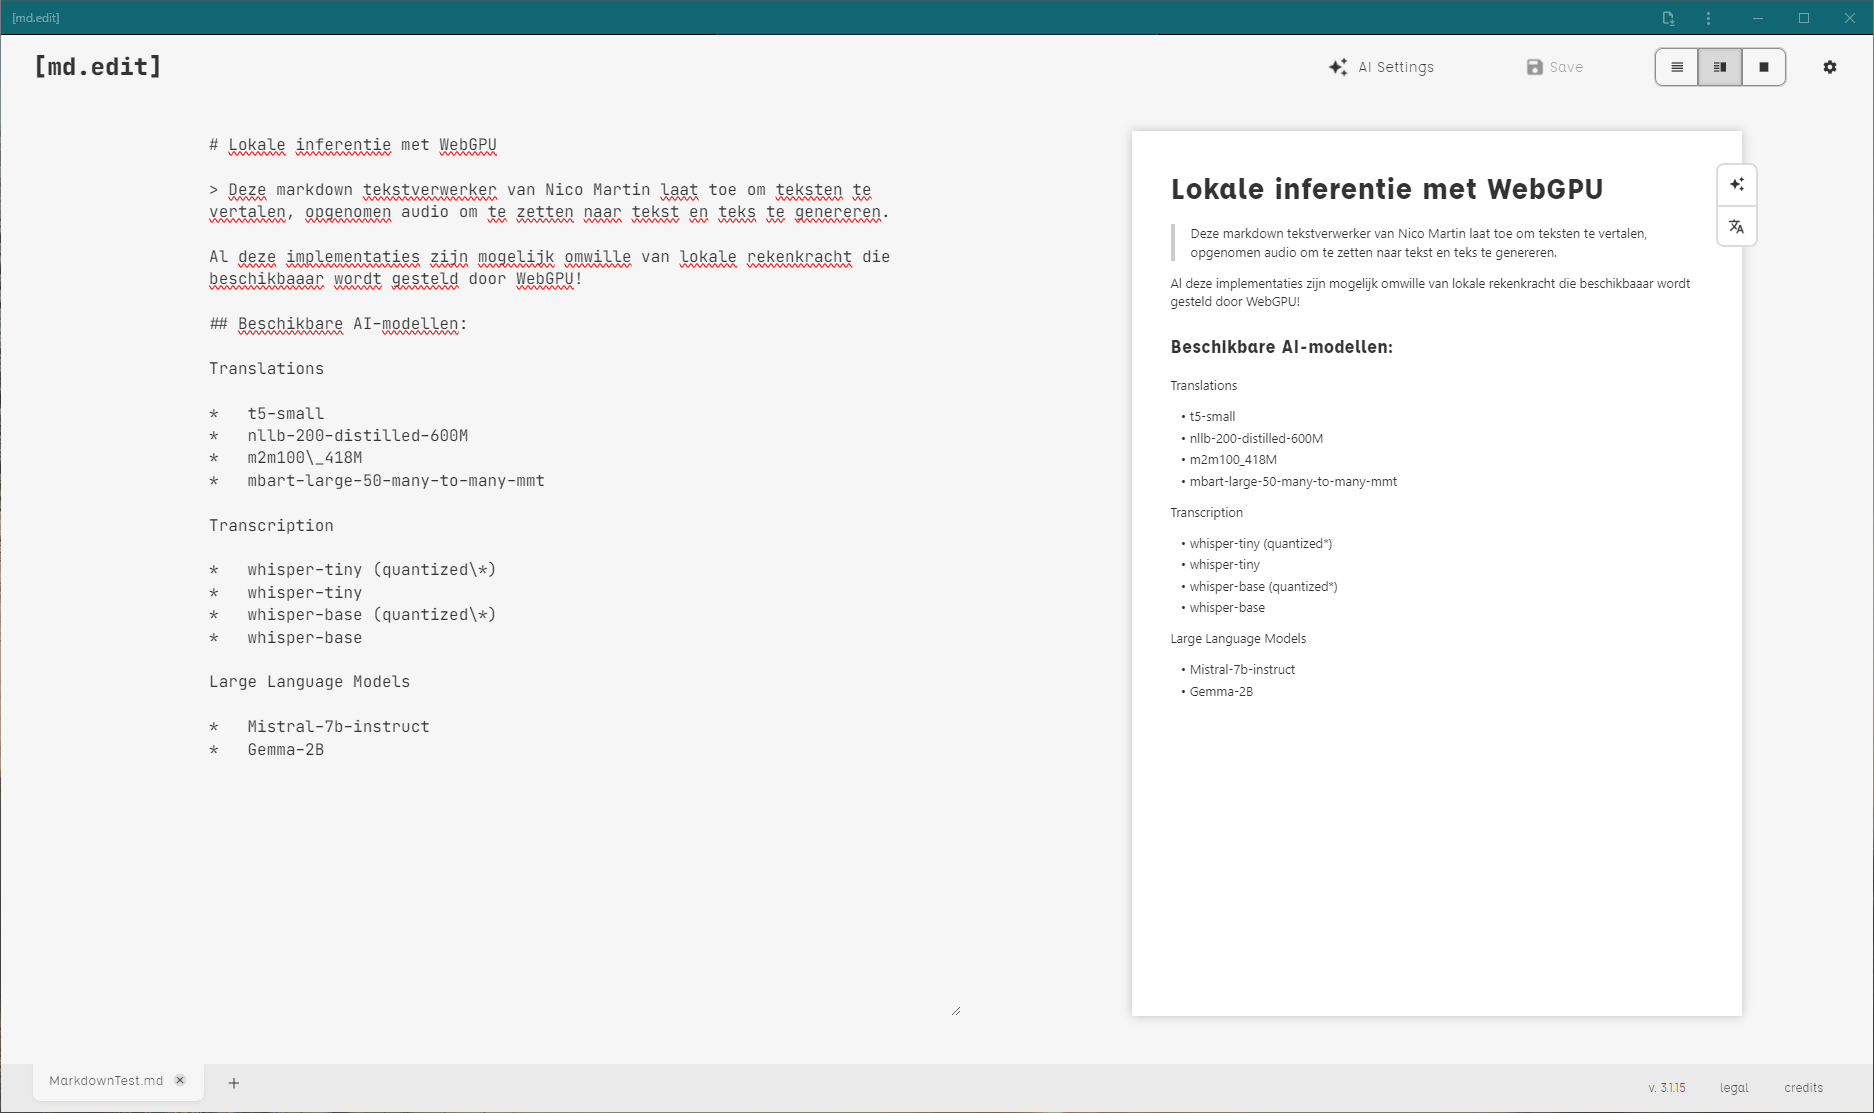
\includegraphics[width=\linewidth]{MarkdownEditor.png}
    \caption[Markdown editor met AI en \textit{WebGPU}~\autocite{Martin2020}]{
        Markdown editor versterkt met kunstmatige intelligentie door middel van \textit{WebGPU}~\autocite{Martin2020}
    }
    \label{fig:MardownEditor}
\end{figure}

\section{Markdown editor}

De \textit{markdown editor} van Nico Martin maakt gebruik van AI-modellen om de functionaliteit van deze \textit{progressive web applicatie} uit te bereiden. \textit{Markdown editor} is een tekstverwerker die toestaat om spraak om te zetten in tekst, dit aan de hand van verschillende versies van \textit{Whisper}~\autocite{radford2022whisper}. Ook worden \textit{large language models} ingezet om delen van tekst te verbeteren of zelfs te vertalen. 

\bigbreak{}

De parallelle rekenkracht van de grafische kaart laat toe dat de browser zelf niet wordt onderbroken. Hierdoor kan de gebruiker ongestoord verder werken en dit maakt de applicatie zeer gebruiksvriendelijk.

\bigbreak{}

Indien deze implementatie geen gebruik zou maken van \textit{WebGPU} zou dit een merkbaar verschil geven op vlak van de snelheid en gebruiksvriendelijkheid. De browser zou op dat moment namelijk gebruik moeten maken van het hoofdproces om  zowel de webapplicatie als de achterliggende AI-modellen te ondersteunen~\autocite{Martin2020}.

\bigbreak{}

In figuur \ref{fig:MardownEditor} wordt de \textit{Markdown editor} van Nico Martin weergegeven in de vorm van een \textit{progressive web application}. De applicatie werd eerst bezocht via de \textit{chrome} browser en hierna simpelweg geïnstalleerd door middel van de installeer knop. Deze knop is beschikbaar wanneer webapplicaties kunnen worden geïnstalleerd als \textit{PWA's}.